\documentclass[utf8x]{beamer}
\usepackage[czech]{babel}
\usepackage{graphics}
\usetheme{Madrid}
\setbeamertemplate{footline}[frame number]
\usepackage{url}
\usepackage{listings}



\title{Hashovací tabulka}
\author{Vladyslav Kovalets}
\institute[xkoval21]{\\Vysoké učenie technické v~Brne \\Fakulta informačních technológií}
\date{\scriptsize{2. 5. 2021}}


\begin{document}

\begin{frame}
  \titlepage
\end{frame}

\begin{frame}{Obsah}
  \tableofcontents
\end{frame}

\section{Co to je}

\subsection{Definice}

\begin{frame}{Definice}
  \begin{itemize}[<+->]
  \item {
    \textbf{Hashovací tabulka} je datová struktura pro ukládání dvojic (klíč, hodnota) nabízející dobrý kompromis mezi rychlostí vyhledávání a paměťovou náročností.
  }

  \item {
    Obecně řečeno, hashovací tabulka je datová struktura se schopností efektivně vkládat, mazat a hledat datové záznamy podle klíče.
  }
  \end{itemize}

\end{frame}

\subsection{Jak to vypadá}
\begin{frame}{Jak to vypadá}

   \begin{figure}[h]

\centering
\scalebox{0.1}{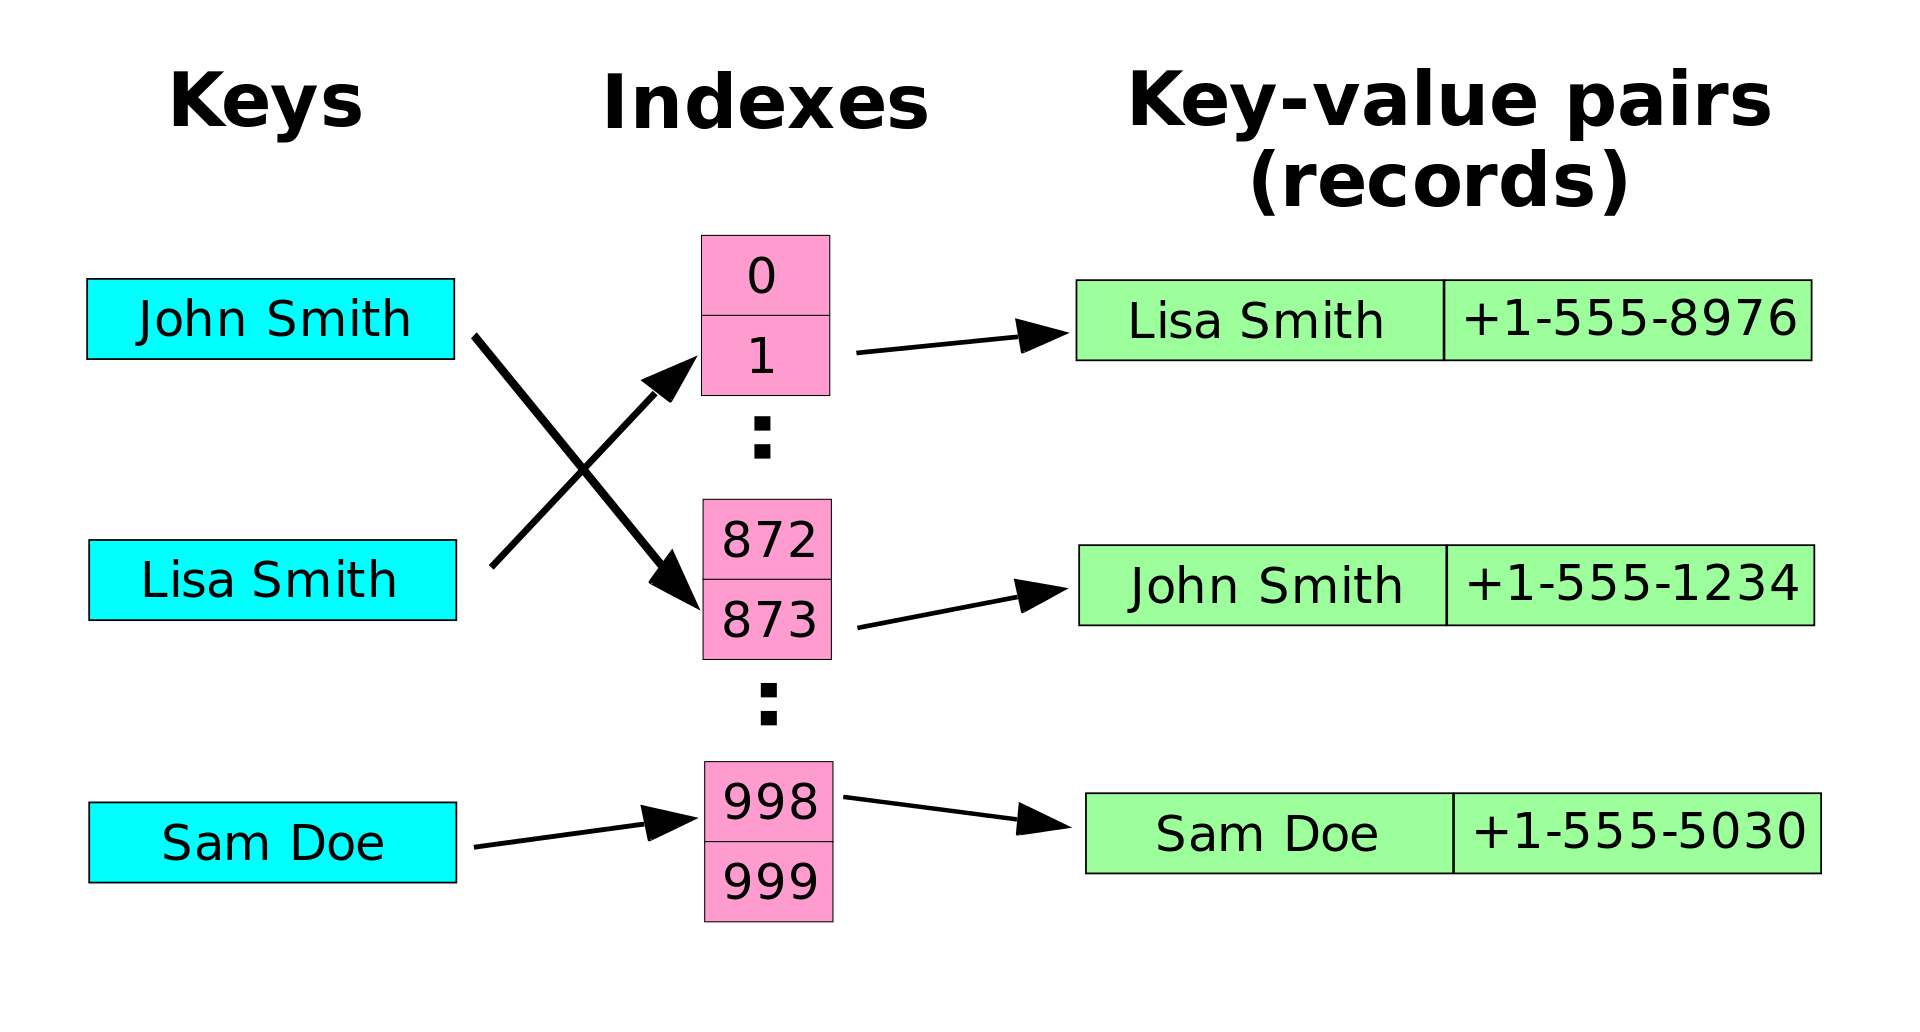
\includegraphics{tabulka.png}}
\caption{Malý telefonní seznam jako hashovací tabulka}

\end{figure}
  \end{frame}
  



\section{Jak to funguje}

\subsection{Princip fungování}

\begin{frame}{Princip fungování}

  Hashovací tabulka uvnitř obsahuje pole tzv. \textbf{slotů}, do kterých lze ukládat záznamy. Hashovací tabulka v podstatě dělá jen to, že na základě klíče vybere vhodný slot a operaci provede v něm. Abychom docílili efektivity, snažíme se, aby všechny sloty byly využity rovnoměrně, tedy aby různé klíče ideálně padaly do různých slotů. Samozřejmě to není zcela možné, protože množina klíčů je mnohem větší než počet slotů. Takové situaci říkáme kolize a existují různé metody, jak tyto kolize řešit:
  \pause
    
  \begin{itemize}[<+->]
  \item {   
    \textbf{zřetězení záznamů} - každý slot obsahuje spojový seznam, do kterého se postupně řetězí prvky patřící do stejného slotu.
  }
  \item {   
     \textbf{otevřená adresace} - obsah všech slotů je umístěn v jednom poli a tak mohou data z jednoho slotu "přetékat" i do jiných slotů a tím zabírat volné místo pro jejich budoucí prvky, což se minimalizuje různými dalšími technikami (linear probing, double hashing...)
  }
  
  \end{itemize}
\end{frame}

\subsection{Asymptotická složitost}

\begin{frame}{Asymptotická složitost}

\begin{table}[]
\begin{tabular}{|l|l|l|}
\hline
\textbf{Operace} & \textbf{Typický případ} & \textbf{Nejhorší případ} \\ \hline
\textit{vyhledávání podle klíče} & \textit{O}(1)         & \textit{O}(n)          \\ \hline
\textit{vkládání záznamu} & \textit{O}(1)         & \textit{O}(n)          \\ \hline
\textit{mazání záznamu} & \textit{O}(1)         & \textit{O}(n)         \\ \hline
\end{tabular}
\end{table}

\end{frame}

\section{Implementace}
\subsection{Pomocí pole}

\begin{frame}{Pomocí pole}

\begin{figure}[h]

\centering
\scalebox{0.3}{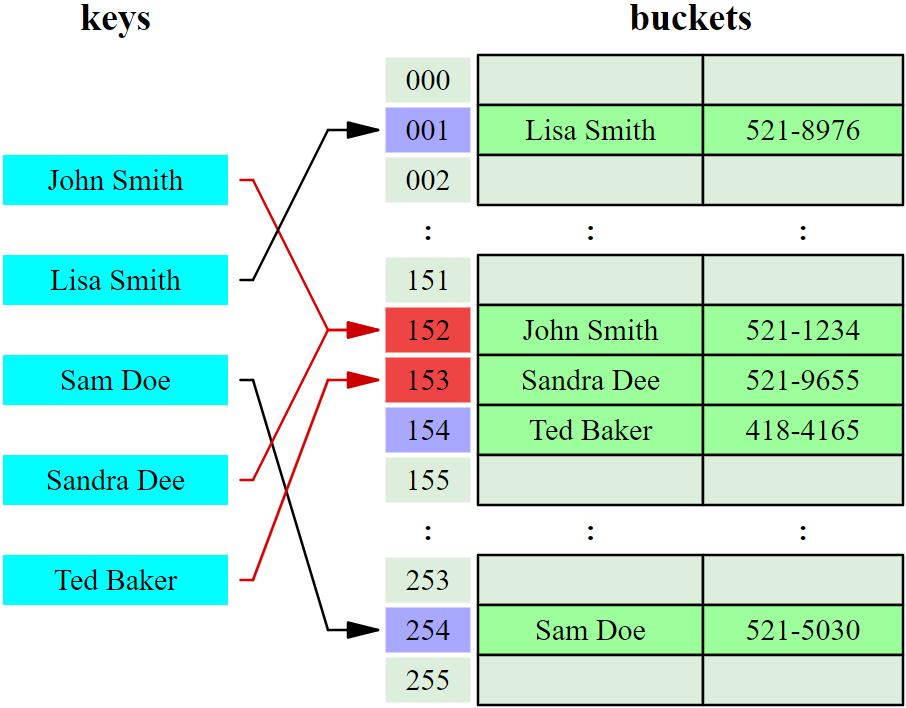
\includegraphics{keys_buckets.jpg}}
\caption{hashovací tabulka realizovaná jedním polem}

\end{figure}

\end{frame}

\begin{frame}{C++ implementace}
\lstinputlisting[language=C]{jazyk_c.c}
\end{frame}

\section{Výhody a nevýhody}


\begin{frame}{Výhody a nevýhody}
    \begin{block}{Výhody}
    \begin{itemize}[<+->]
    
    	\item{hašování je v porovnání s jinými vyhledávacími metodami, např. vyhledávacími stromy (nejen binárními), v průměrném případě asymptoticky rychlejší.}
    	
    \end{itemize}
    \end{block}
    
    \begin{block}{Nevýhody}
     \begin{itemize}[<+->]
     
        \item { neposkytuje záruky pro nejhorší případ.}
		
        \item {potřebuje úplný klíč, tj. neumožňuje dobré vyhledávání pro částečně známý klíč pro strukturované klíče nebo klíče ve vícerozměrném prostoru.}
        
        \item {neposkytuje intervalové dotazy, tj. vyhledání všech klíčů v daném intervalu.}
         \end{itemize}
        
    \end{block}
\end{frame}

\appendix

\begin{frame}{Použité zdroje}
\begin{thebibliography}{}

\bibitem{} Voho.eu:
    \emph{Hashovací tabulka}. [online], [citováno 2. 5. 2021].\\
    Dostupné z: \texttt{http://voho.eu/wiki/datova-struktura-hash-tabulka/}
\vspace{2mm}
\bibitem{} Wikipedia.org:
    \emph{Hašovací tabulka}. [online], [citováno 2. 5. 2021].\\
    Dostupné z: \texttt{https://cs.wikipedia.org/wiki/Hašovací\_tabulka}

\end{thebibliography}
\end{frame}
\end{document}